\section{LDAP Server Confirmation}
\label{appendix:ldap_server_confirmation}
\begin{table}[!hb]
\centering
\footnotesize
\setlength\tabcolsep{4pt}
\begin{tabular}{@{} l rr p{0cm} rr @{}} 
\toprule
\thead{LDAP Error} & \multicolumn{2}{c}{\thead{Port 389}}  && \multicolumn{2}{c}{\thead{Port 636}} \\
\cline{2-3}\cline{5-6}
\thead{Result Codes} & \multicolumn{1}{c}{\thead{v2}} &  \multicolumn{1}{c}{\thead{v3}} && \multicolumn{1}{c}{\thead{v2}}& \multicolumn{1}{c}{\thead{v3}}\\
\midrule
\midrule
authMethodNotSupported        & 4 & 4 && 19 & 19 \\
authorizationDenied           & 2 & 2 && - & - \\
confidentialityRequired       & 12 & 100 && - & - \\
inappropriateAuthentication   & 2,810 & 7,578 && 487 & 3,636 \\
insufficientAccessRights      & 98 & 330 && - & 145 \\
invalidCredentials            & 1,159 & 1,154 && 1,497 & 1,575 \\
invalidDNSyntax               & 10 & 10 && 1 & 1 \\
namingViolation               & - & 6 && - & 8 \\
operationsError               & 87 & 102 && 3 & 15 \\
protocolError                 & 32,353 & 56 && 12,870 & - \\
strongerAuthRequired          & 3 & 3 && - & - \\
timeLimitExceeded             & - & 18 && - & 1 \\
unavailable                   & 1 & 1 && - & 1 \\
unwillingToPerform            & 44 & 68 && 97 & 93 \\
%[0.4em]
%\midrule
%Client-side                   &&&&& \\
%SERVER\_DOWN                  & 105 & 124 && 54 & 48 \\
%TIMEOUT                       & 148 & 38 && 9 & 4 \\
%None                            & 44132 & 71374 && 19058 & 28549 \\
\bottomrule
\end{tabular}
\caption{LDAP error result codes.}
\label{tab:ldap_error_messages}
\end{table}

%We document the errors for failed LDAPv2 and LDAPv3 binds in \cref{tab:ldap_error_messages}. 
\cref{tab:ldap_error_messages} shows the errors for failed LDAPv2 and LDAPv3 binds. We observe that the majority of LDAPv2 bind requests were met with a \texttt{protocolError} response, indicating dwindling legacy support. Servers also commonly disallow anonymous binds (\texttt{inappropriateAuthentication}) or mark empty credentials as invalid (\texttt{invalidCredentials}).


\section{Categorization of Servers}
\begin{table}[tb!]
\centering
\footnotesize
\setlength{\tabcolsep}{5pt}
\begin{tabular}{@{}l r r r r@{}}
\toprule
\thead{Server Types}& \thead{Total}  & \thead{OID}  & \thead{Version}  & \thead{Attributes} \\
                              %& \thead{ \#IPs}  & \thead{ \#IPs}  & \thead{ \#IPs}  & \thead{\#IPs} \\
\midrule
\midrule
Linux User Man. & 5,180 & 0 & 0 & 5,180 \\
Microsoft Active Dir. & 4,465 & 4,465 & 0 & 51 \\
Sun Java System Dir. & 1,818 & 1,818 & 0 & 0 \\
iPlanet Directory & 1,592 & 1,592 & 0 & 0 \\
Apple Schema for AD & 1,387 & 0 & 0 & 1,387 \\
389 Directory Server & 1,348 & 0 & 1,348 & 0 \\
Apple with OpenLDAP & 574 & 0 & 574 & 0 \\
ApacheDS & 171 & 0 & 171 & 0 \\
DICOM & 145 & 0 & 0 & 145 \\
HL7 & 141 & 0 & 0 & 141 \\
\bottomrule
\end{tabular}
\caption{Overview of the top 10 categorized server types and the categorization methods.}
\label{tab:CatResults}
\end{table}
We have categorized the LDAP servers based on the OIDs they expose, their version number, and the attributes they use. Table \ref{tab:CatResults} shows the top 10 list of all categorized server types.


\section{Personal Data Attribute Groups}
\label{appendix:attribute_anaylsis}
We have extracted all attributes from the LDAP samples that potentially contain personal data and categorized them into general groups. The classification of the identified attributes into groups is shown in Table \ref{tab:personal_data_attribute_groups}.
% \begin{table*}[tb]
% \setlength\tabcolsep{2pt}
%     \small
%     \centering
%     \begin{tabularx}{\textwidth}{@{} l X @{}}
%     \toprule
%         \thead{Personal Data} & \thead{LDAP Attributes} \\
%         \thead{Group} &  \\
%         \midrule
%         \midrule
%         Last Name & lastName, LastName, sn, sn;lang-cs, sn;lang-en, sn;lang-ja, sn;lang-el sn;x-role-2, uvmEduSurname, i3sicLastName, suDisplayNameLast \\
%         Email & EMAIL, eMailAddress, email, i3sicEmail, mail, mailAlias, mailAlternateAddress, mailLocalAddress, mailalias, zimbraMailAlias, umMailAlias, umAlternateMail, suMailAddress, mailAliasLast, mailAliasLastLaw, mailAliasesLaw, mailAliases \\
%         First Name & firstName, FirstName, givenName, givenName;lang-cs, givenName;lang-ja, givenName;lang-el, givenName;x-role-2, givenname, i3sicFirstName, middleName, umDisplayFirstName, suDisplayNameFirst, suDisplayNameMiddle, umMiddleInitial, ucMiddleName, cuMiddlename \\
%         Full Name & displayName, displayname, eduPersonNickname, umDisplayName, umDisplayNameLF, krbPrincipalName, username, nsNickName, umNickName, nsnickname, mozillaNickname, nickname,  fullName, name, CallerIDName, suDisplayNameLF, umNameComponent, suOtherName \\
%         Birthday& apple-birthday, birthDay, dateOfBirth, schacDateOfBirth, birthDate \\
%         Gender & gender, sex, schacGender \\
%         Country & c, co, countryCode, state, st, country, userCountry, mozillaHomeState \\
%         Phone Number & homePhone, telephoneNumber, uvmEduOfficePhone, mobile, i3sicLocalPhoneNumber, facsimileTelephoneNumber, MobileNumber, HomeNumber, suGwAffilPhone1, telephonenumber, otherTelephone, osuAltPhoneNumber, otherMobile, phone \\
%         Address &  homePostalAddress, streetAddress, street, postalAddress, uvmEduOfficeAddress, umStreetAddress, suGwAffilAddress1, mozillaHomeStreet, postalAddress;x-role-2, osuOfficeAddress, mozillaHomeStreet2 \\
%         Location & l, location, uvmEduOfficeLocation, mozillaHomeLocalityName, provinceName, postalCode, zip, city \\
%         Public Key & userCertificate, userCertificate;binary, pgpKey, nDSPKIPublicKeyCertificate, nDSPKIPublicKey, userPKCS12, userSMIMECertificate \\
%         Title &  isDoctor, title, title;x-role-2, personalTitle, umOfficialTitle, umDisplayTitle, umPrimaryTitle, umNamePrefix, umNameSuffix, suDisplayNamePrefix, suDisplayNameSuffix \\
%         Job & company, department, employeeNumber, employeeType, umEmployee, eduPersonAffiliation, eduPersonPrimaryAffiliation, Department, umPrimaryDeptName, umPrimaryInstitutionCode, umInstitutionCode, umPrimaryInstitution, umDepartment, suGwAffiliation2, suDisplayAffiliation, suGwAffiliation1, suAffiliation, ucDepartment, departmentName, osuPrimaryAffiliation, osuDepartment, companyName, brEduAffiliation, psDepartment, hireDate \\
%         Photo & jpegPhoto, photograph \\
%         SSN & socialSecurityNumber \\
%     \bottomrule
%     \end{tabularx}
% \caption{Grouping of LDAP attributes containing personal data.}
% \label{tab:personal_data_attribute_groups}
% \end{table*}


\begin{table}[!htb]
\setlength\tabcolsep{1pt}
\renewcommand{\arraystretch}{1.3}
    \footnotesize
    \centering
    \begin{tabularx}{\linewidth}{@{} X @{}}
    \toprule
        \thead{Personal Data Group} LDAP Attributes\\
        \midrule
        \midrule
        \textbf{Last Name}  lastName, LastName, sn, sn;lang-cs, sn;lang-en, sn;lang-ja, sn;lang-el sn;x-role-2, uvmEduSurname, i3sicLastName, suDisplayNameLast \\
        \textbf{Email}  EMAIL, eMailAddress, email, i3sicEmail, mail, mailAlias, mailAlternateAddress, mailLocalAddress, mailalias, zimbraMailAlias, umMailAlias, umAlternateMail, suMailAddress, mailAliasLast, mailAliasLastLaw, mailAliasesLaw, mailAliases \\
        \textbf{First Name}  firstName, FirstName, givenName, givenName;lang-cs, givenName;lang-ja, givenName;lang-el, givenName;x-role-2, givenname, i3sicFirstName, middleName, umDisplayFirstName, suDisplayNameFirst, suDisplayNameMiddle, umMiddleInitial, ucMiddleName, cuMiddlename \\
        \textbf{Full Name}  displayName, displayname, eduPersonNickname, umDisplayName, umDisplayNameLF, krbPrincipalName, username, nsNickName, umNickName, nsnickname, mozillaNickname, nickname,  fullName, name, CallerIDName, suDisplayNameLF, umNameComponent, suOtherName \\
        \textbf{Birthday} apple-birthday, birthDay, dateOfBirth, schacDateOfBirth, birthDate \\
        \textbf{Gender}  gender, sex, schacGender \\
        \textbf{Country}  c, co, countryCode, state, st, country, userCountry, mozillaHomeState \\
        \textbf{Phone}  homePhone, telephoneNumber, uvmEduOfficePhone, mobile, i3sicLocalPhoneNumber, facsimileTelephoneNumber, MobileNumber, HomeNumber, suGwAffilPhone1, telephonenumber, otherTelephone, osuAltPhoneNumber, otherMobile, phone \\
        \textbf{Address}   homePostalAddress, streetAddress, street, postalAddress, uvmEduOfficeAddress, umStreetAddress, suGwAffilAddress1, mozillaHomeStreet, postalAddress;x-role-2, osuOfficeAddress, mozillaHomeStreet2 \\
        \textbf{Location}  l, location, uvmEduOfficeLocation, mozillaHomeLocalityName, provinceName, postalCode, zip, city \\
        \textbf{Public Key}  userCertificate, userCertificate;binary, pgpKey, nDSPKIPublicKeyCertificate, nDSPKIPublicKey, userPKCS12, userSMIMECertificate \\
        \textbf{Title}   isDoctor, title, title;x-role-2, personalTitle, umOfficialTitle, umDisplayTitle, umPrimaryTitle, umNamePrefix, umNameSuffix, suDisplayNamePrefix, suDisplayNameSuffix \\
        \textbf{Job}  company, department, employeeNumber, employeeType, umEmployee, eduPersonAffiliation, eduPersonPrimaryAffiliation, Department, umPrimaryDeptName, umPrimaryInstitutionCode, umInstitutionCode, umPrimaryInstitution, umDepartment, suGwAffiliation2, suDisplayAffiliation, suGwAffiliation1, suAffiliation, ucDepartment, departmentName, osuPrimaryAffiliation, osuDepartment, companyName, brEduAffiliation, psDepartment, hireDate \\
        \textbf{Photo}  jpegPhoto, photograph \\
        \textbf{SSN}  socialSecurityNumber \\
    \bottomrule
    \end{tabularx}
\caption{Personal data attribute groups.}
\label{tab:personal_data_attribute_groups}
\end{table}





\section{Analysis of TLS and X.509}

\label{appendix:tls}

\begin{table*}[!tb]
\centering
\footnotesize
\begin{tabular}{@{}lrrrrrr@{}}
\toprule
 & \thead{Total IPs} & \thead{Leak credentials} & \thead{Personal data}  & \thead{SASL support}   & \thead{CVE} & \thead{Internal info.} \\ 
\midrule
\midrule
Supporting TLS & 48,198 (100\%) & 910 (100\%) & 7,378 (100\%) & 18,502 (100\%) & 528 (100\%) & 7,118 (100\%) \\
\arrayrulecolor{gray!90}
\midrule
\arrayrulecolor{black}
TLSv1.3 & 36.67\% & 20.00\% & 27.24\% & 42.04\% & 28.41\% & 49.34\% \\
TLSv1.2 & 59.46\% & 77.03\% & 68.91\% & 55.92\% & 71.59\% & 46.90\% \\
TLSv1.1 & 0.33\%  & 0.33\%  & 0.16\%  & 0.23\%  & 0.00\%  & 0.10\% \\
TLSv1.0 & 3.54\%  & 2.64\%  & 3.69\%  & 1.81\%  & 0.00\%  & 3.67\% \\
\midrule
\arrayrulecolor{black}
Recommended cipher suites           & 65.92\%       & 36.59\%          & 44.20\%       & 57.49\%       & 94.89\%     & 61.42\%        \\
Other cipher suites        & 34.08\%       & 63.41\%          & 55.80\%       & 42.51\%       & 5.11\%      & 38.58\%        \\
\ldots with RSA key exchange & 24.27\%       & 57.14\%          & 53.71\%       & 41.77\%       & 5.11\%      & 36.93\%        \\
\ldots using CBC           & 12.26\%       & 8.35\%           & 6.30\%         & 3.64\%        & 5.11\%      & 5.49\%         \\
\ldots using 3DES               & 0.31\%        & 0.00\%           & 0.03\%        & 0.00\%        & 0.00\%      & 0.00\%        \\
\midrule
\arrayrulecolor{black}
Valid Cert. Chain                    & 36.81\% & 17.69\% & 24.10\% & 40.38\% & 32.20\% & 47.78\% \\
Invalid Cert. Chain                   & 63.19\% & 82.31\% & 75.90\% & 59.62\% & 67.80\% & 52.22\% \\
... Self-signed           & 32.30\% & 21.87\% & 22.61\% & 16.53\% & 1.70\% & 10.97\% \\
... Expired/not yet valid & 19.65\% & 43.63\% & 35.52\% & 25.15\% & 6.63\% & 14.34\% \\
... Unknown authority     & 11.20\% & 16.70\% & 17.74\% & 17.91\% & 59.28\% & 26.89\% \\
\bottomrule
\end{tabular}
\caption{Overview of the results of the Network Analysis Module.}
\label{tab:tls_overview}
\end{table*}

%\todo{Cross-check against tables!!! This was written before the final tables were in. And check with Section 6 !!}

%\todo{We are going to update \cref{tab:ciphersuites} such that it summarizes in two categories.}

%\todo{The problem with ``static'' IPs again. What is our argument that we use the ``static'' hosts as a reference number? In reality, it is because we did not have FHM's IPs from their zmap scans early because those scans were still. But we could now filter for that to avoid this entire problem.} Our TLS analysis for cipher suites and X.509 certificate validation aggregate datasets and filter by hosts that negotiated and we retrieved their TLS certificates, forming a subset of the hosts expressed in \cref{tab:results_overview}.

% this 56k are from UT scans; stable LDAP servers (servers that appear in more than one scan, over time)
Only about 60\% (56k) of the candidate hosts respond to our scans with a successful \acrshort{TLS} connection. This is expected: recent findings by Sattler \etal~\cite{Sattler2023} and Izhikevich \etal~\cite{Izhikevich2022} show that many IPv4 addresses respond to a SYN packet but do not follow through with a full TCP handshake.

%\todo{Cross-check against tables!!!}
\paragraph{TLS Versions.} \acrshort{TLS} 1.3 experienced an unusually fast deployment on the Web, in part because of the widespread use of cloud hosting~\cite{Holz2020}. After just a few years, the deployment already exceeded 30\%. We also find substantial deployment of this version (which mandates many strong security features) also for \acrshort{LDAP}, with deployment at nearly 37\% of all analyzed hosts. Once again, the numbers are significantly lower for the servers that leak information---and better for those that support authentication. Still, TLS 1.2, which has come under significant pressure in recent years, is still by far the most widely deployed version, especially for servers with data leakages.


\paragraph{Cipher Suites.} Numerous cipher suites are defined for use in \acrshort{TLS}. They indicate the symmetric cipher, block mode (if applicable), and the hash algorithm for the \gls{MAC}. In addition, they indicate how the session key for the symmetric cipher is to be derived. In our evaluation, we generally refer to RFC 9325~\cite{rfc9325}, which defines best practices for \acrshort{TLS}. In particular, this means that the key exchange should be ephemeral Diffie-Hellman (DHE) to enable forward security, ideally on elliptic curves. Classic finite-field Diffie-Hellman is discouraged for \acrshort{TLS} 1.2, and non-ephemeral Diffie-Hellman is generally viewed as too weak. Using RSA in the key exchange means that forward secrecy is not possible; the RFC advises strongly against this.

RSA can be used for authentication. In this case, the RFC requires the key to be at least 2048 bit long.  Concerning block ciphers, the RFC views \acrfull{GCM} as secure, whereas \gls{CBC} is under pressure due to padding oracle attacks~\cite{_PaddingOraclesDecline_2016} possible in some contexts. This can be mitigated when \gls{CBC} is negotiated with the ``encrypt\_then\_mac'' \acrshort{TLS} extension. However, none of the major \gls{LDAP} clients we tested sent this extension. Therefore, we excluded it from our scans.
Older hashing algorithms such as SHA1 are deprecated; the more modern SHA2 and SHA3 or the Poly1305 family of hash functions should be used instead. 
The effective length of the symmetric session keys should never be less than 128 bits; the RFC explicitly mentions 3DES as an example of a cipher with insufficient key length.
We implemented the most relevant parts of RFC~9325 to evaluate the use of \acrshort{TLS} in our data set. 
%We categorized the following ciphers with the help of the RFC: TLS\_AES\_128\_GCM\_SHA256, TLS\_AES\_256\_GCM\_SHA384, TLS\_CHACHA20\_POLY1305\_SHA256, TLS\_ECDHE\_ECDSA\_WITH\_AES\_128\_GCM\_SHA256, TLS\_ECDHE\_ECDSA\_WITH\_AES\_256\_GCM\_SHA384, TLS\_ECDHE\_RSA\_WITH\_AES\_128\_CBC\_SHA256, TLS\_ECDHE\_RSA\_WITH\_AES\_128\_GCM\_SHA256, TLS\_ECDHE\_RSA\_WITH\_AES\_256\_GCM\_SHA384, TLS\_ECDHE\_RSA\_WITH\_CHACHA20\_POLY1305\\\_SHA256, TLS\_ECDHE\_ECDSA\_WITH\_CHACHA20\\\_POLY1305\_SHA256.
%Another limitation is that our scanner cannot determine whether \gls{ECDSA} is signed following the recommendation using NIST curve P-256. Similarly, we cannot detect the key size when DHE or ECDHE is exchanged to give a better verdict on the security of such key exchange methods.

\cref{tab:tls_overview} summarizes our findings. 
We find that a decent number of connections (around 65\%) use one of the recommended cipher suites. Across all \acrshort{TLS}-supporting \acrshort{LDAP} instances, we find that AES-GCM is widely used, often even with a secure key length of 256 bit. The modern stream cipher ChaCha20 is in significant use as well (20\%). However, servers that leak credentials commonly use recommended cipher suites significantly less frequently. The same is true for server versions for which we find at least one CVE and, to a lesser degree, also for servers that contain personal data. Servers that provide support for \acrfull{SASL} or hold internally relevant, security-critical information, however, tend to be more commonly configured with better cryptography. Yet, this is still unsatisfactory: for example, 38\% of servers that hold information of the latter kind still use cipher suits besides the recommended ones. Overall, this paints a picture where weaker cryptography correlates with leakages of sensitive data.

\iffalse
cipher\_name	                                    recommended	percentage
TLS\_CHACHA20\_POLY1305\_SHA256	                    Y	        16.70
TLS\_ECDHE\_ECDSA\_WITH\_CHACHA20\_POLY1305\_SHA256	Y	        0.39
TLS\_ECDHE\_RSA\_WITH\_CHACHA20\_POLY1305\_SHA256	N	        0.08
TLS\_ECDHE\_RSA\_WITH\_CHACHA20\_POLY1305\_SHA256	Y	        2.80
\fi

\iffalse
summary:
- on clients not in general, the not-rec:
TLS\_RSA\_WITH\_AES\_128\_CBC\_SHA256
TLS\_ECDHE\_RSA\_WITH\_AES\_128\_CBC\_SHA256
- on clients not in general, the rec:
TLS\_ECDHE\_RSA\_WITH\_AES\_128\_CBC\_SHA256
- all in general are on clients

\begin{tabular}{ll}
\toprule
cipher\_name & recommended \\
\midrule
TLS\_ECDHE\_RSA\_WITH\_AES\_256\_CBC\_SHA & N \\
TLS\_RSA\_WITH\_AES\_256\_GCM\_SHA384 & N \\
TLS\_RSA\_WITH\_AES\_256\_CBC\_SHA & N \\
TLS\_RSA\_WITH\_AES\_128\_GCM\_SHA256 & N \\
TLS\_RSA\_WITH\_AES\_128\_CBC\_SHA & N \\
TLS\_ECDHE\_RSA\_WITH\_AES\_256\_GCM\_SHA384 & N \\
TLS\_ECDHE\_RSA\_WITH\_CHACHA20\_POLY1305\_SHA256 & N \\  % <-- revD said this is OK
TLS\_ECDHE\_RSA\_WITH\_AES\_128\_GCM\_SHA256 & N \\
TLS\_RSA\_WITH\_3DES\_EDE\_CBC\_SHA & N \\
TLS\_ECDHE\_RSA\_WITH\_AES\_128\_CBC\_SHA & N \\
TLS\_ECDHE\_ECDSA\_WITH\_CHACHA20\_POLY1305\_SHA256 & Y \\  % <-- revD said this is OK
TLS\_ECDHE\_RSA\_WITH\_AES\_256\_GCM\_SHA384 & Y \\
TLS\_ECDHE\_RSA\_WITH\_CHACHA20\_POLY1305\_SHA256 & Y \\ % <-- revD said this is OK
TLS\_ECDHE\_ECDSA\_WITH\_AES\_256\_GCM\_SHA384 & Y \\
TLS\_ECDHE\_ECDSA\_WITH\_AES\_128\_GCM\_SHA256 & Y \\
TLS\_CHACHA20\_POLY1305\_SHA256 & Y \\
TLS\_AES\_256\_GCM\_SHA384 & Y \\
TLS\_ECDHE\_RSA\_WITH\_AES\_128\_GCM\_SHA256 & Y \\
TLS\_AES\_128\_GCM\_SHA256 & Y \\
\bottomrule
\label{tab:aggr_all_rec_ciphers}
\caption{Aggregation of all 6 datasets, with unique ciphername, recommendation}
\end{tabular}

\begin{tabular}{ll}
\toprule
cipher\_name & recommended \\
\midrule
TLS\_ECDHE\_RSA\_WITH\_AES\_128\_CBC\_SHA & N \\
TLS\_RSA\_WITH\_3DES\_EDE\_CBC\_SHA & N \\
TLS\_RSA\_WITH\_AES\_256\_CBC\_SHA & N \\
TLS\_RSA\_WITH\_AES\_128\_GCM\_SHA256 & N \\
TLS\_RSA\_WITH\_AES\_128\_CBC\_SHA256 & N \\
TLS\_RSA\_WITH\_AES\_128\_CBC\_SHA & N \\
TLS\_RSA\_WITH\_AES\_256\_GCM\_SHA384 & N \\
TLS\_ECDHE\_RSA\_WITH\_AES\_256\_GCM\_SHA384 & N \\
TLS\_ECDHE\_RSA\_WITH\_AES\_256\_CBC\_SHA & N \\
TLS\_ECDHE\_RSA\_WITH\_AES\_128\_GCM\_SHA256 & N \\
TLS\_ECDHE\_RSA\_WITH\_AES\_128\_CBC\_SHA256 & N \\
TLS\_ECDHE\_RSA\_WITH\_CHACHA20\_POLY1305\_SHA256 & N \\ % <-- revD said this is OK
TLS\_AES\_128\_GCM\_SHA256 & Y \\
TLS\_AES\_256\_GCM\_SHA384 & Y \\
TLS\_CHACHA20\_POLY1305\_SHA256 & Y \\
TLS\_ECDHE\_ECDSA\_WITH\_AES\_128\_GCM\_SHA256 & Y \\
TLS\_ECDHE\_ECDSA\_WITH\_AES\_256\_GCM\_SHA384 & Y \\
TLS\_ECDHE\_RSA\_WITH\_AES\_128\_CBC\_SHA256 & Y \\
TLS\_ECDHE\_RSA\_WITH\_AES\_128\_GCM\_SHA256 & Y \\
TLS\_ECDHE\_RSA\_WITH\_AES\_256\_GCM\_SHA384 & Y \\
TLS\_ECDHE\_RSA\_WITH\_CHACHA20\_POLY1305\_SHA256 & Y \\ % <-- revD said this is OK
TLS\_ECDHE\_ECDSA\_WITH\_CHACHA20\_POLY1305\_SHA256 & Y \\ % <-- revD said this is OK
\bottomrule
\label{tab:aggr_ldapclients_rec_ciphers}
\caption{Aggregation of all five LDAP clients, with unique cipher name, recommendation}
\end{tabular}
\fi

% THIS IS DUPLICATED, CLIENT HELLO IS ON SEC 6
%\paragraph{LDAP clients cipher suites.} We targeted and passively monitored the University's LDAP server to obtain the client hello parameters of major \acrlong{LDAP} client.  We conducted additional scans using crafted client-hello replicating such \acrshort{LDAP} clients to obtain insights into their \acrshort{TLS} posture by what cipher suites LDAP servers would select. We used our analysis described earlier to categorize recommended cipher suites. We summarize it in \cref{tab:ClientHelloCipherSuites} considering the aforementioned limitations.

%Additionally, our scanner does not support some cipher suites the clients offer to exchange. We evaluated them and found that these cipher suites use ephemeral DH, \gls{CBC} mode for encryption, or RSA for key exchange. For compatibility reasons, the clients, except for Thunderbird and LDAP administrator, also offer TLS\_EMPTY\_RENEGOTIATION\_INFO\_SCSV. In summary, none of these cipher suites improve the connection security when used to connect to LDAP servers.

%used in a TLS connection between client and server. The goal is to ensure communication confidentiality, data integrity, and server authenticity. Cipher suites tell, in a TLS session, the key exchange algorithms used to share the session secret key, the algorithm used to authenticate the server's identity, the encryption, and the hash algorithms used.

%We compare static LDAP servers with those where we found different categories of issues, as presented earlier.  Concerning non-recommended cipher suites, LDAP servers chose various forms of weak key exchange, authentication, encryption, and hash algorithms. For instance, key exchange using RSA is not recommended as it does not offer forward secrecy (\eg "TLS\_RSA\_WITH\_AES\_128\_GCM\_SHA256")~\cite{rfc9325}.

% When RSA is used to authenticate the server's identity (\eg "TLS\_ECDHE\_RSA\_WITH\_AES\_128\_GCM\_SHA256"), it is also recommended to use a certificate with at least 2048 bits of public key, which we see that a few servers do not follow. Encryption with AES in Cipher Block Chaining (CBC) stream cipher is also considered insecure (\eg "TLS\_RSA\_WITH\_AES\_128\_CBC\_SHA") as it is proven to be exploitable at the padding oracle attack~\cite{_PaddingOraclesDecline_2016}.

% Finally, SHA1 is considered insecure as collisions were~\cite{WangEtAlCollisionsSha1} found and have been declared deprecated since 2011 by NIST. 
% https://csrc.nist.gov/news/2022/nist-transitioning-away-from-sha-1-for-all-apps \cite{ComputerSecurityDivision_NISTTransitioningAway_2022}

\iffalse
\begin{figure}
    \centering
    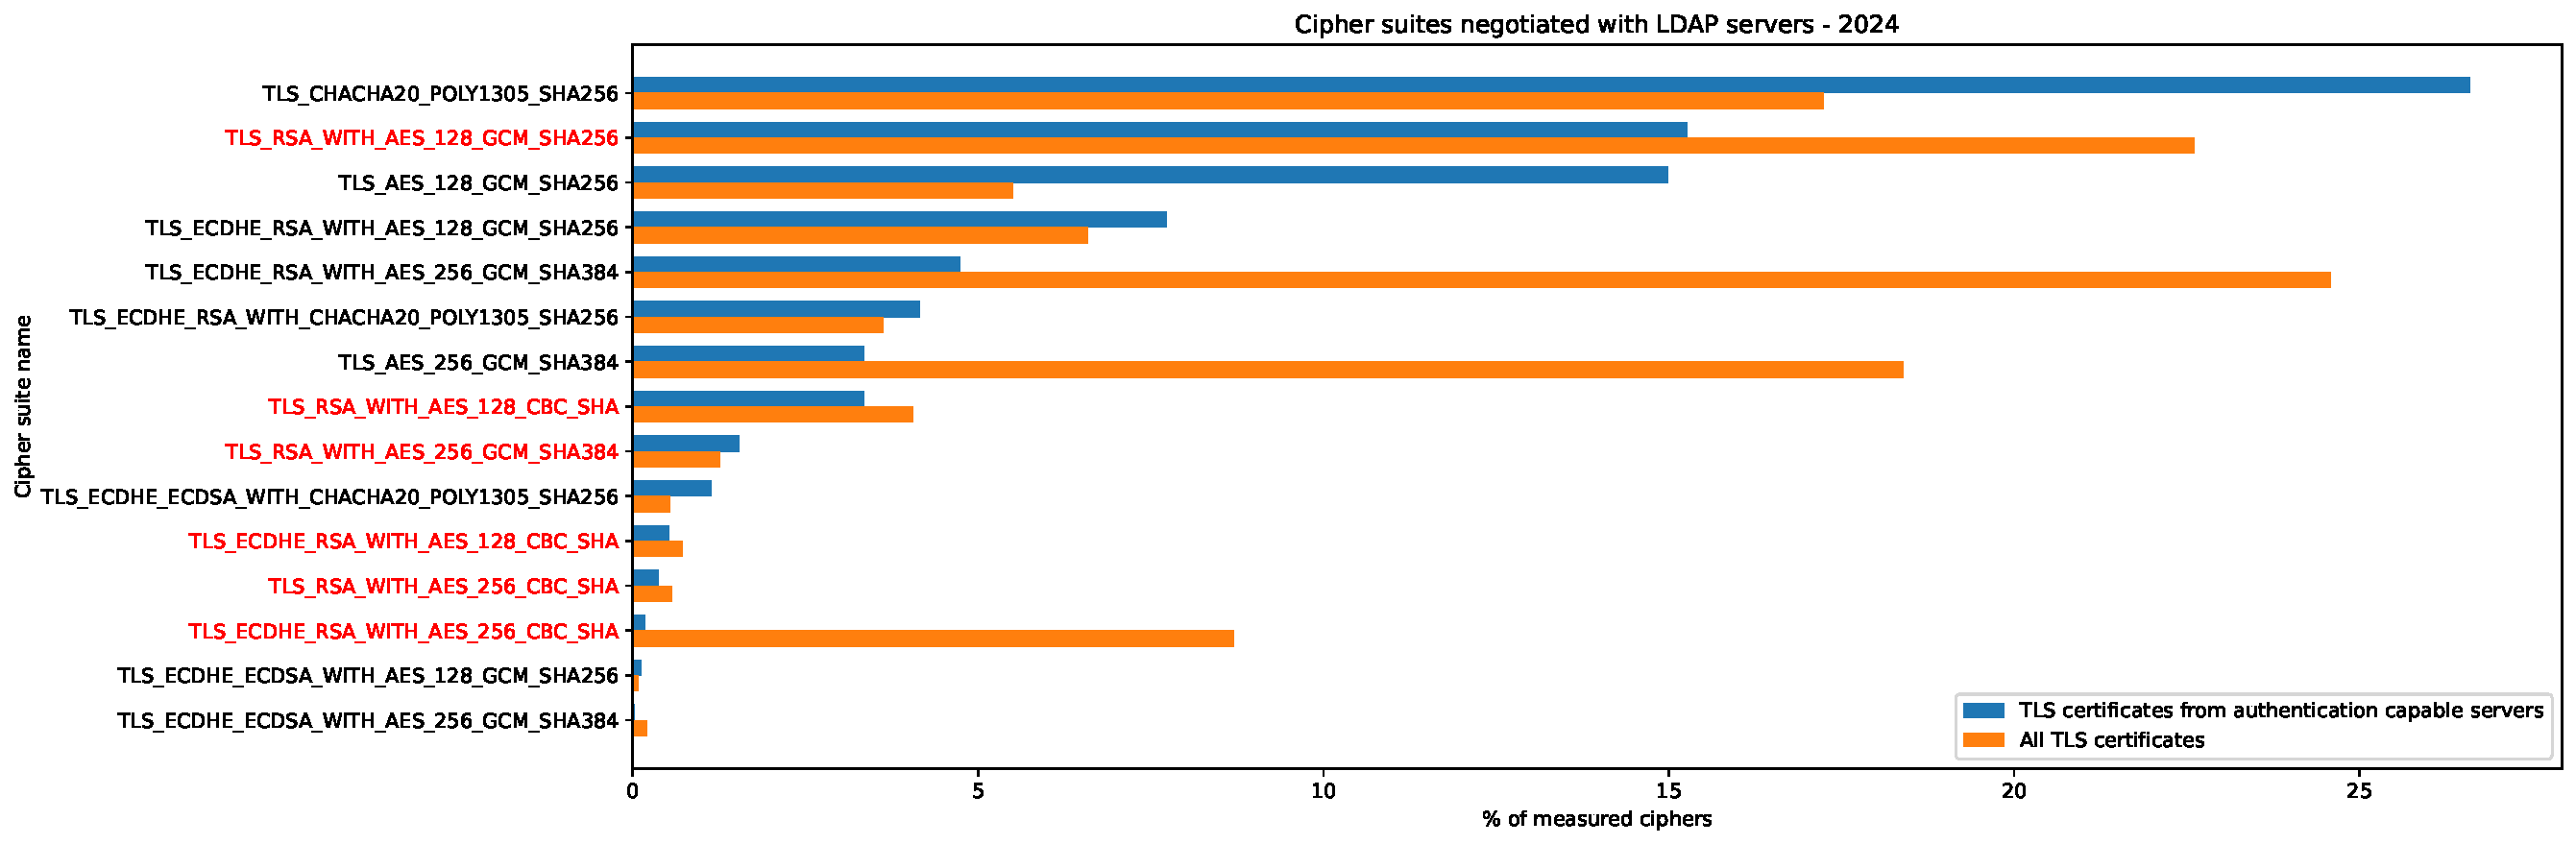
\includegraphics[width=0.47\textwidth]{img/cipher_suites.pdf}
    \caption{Cipher suites in TLS communication of LDAP servers.}
    \label{fig:cipher_suites}
\end{figure}
\paragraph{PII in plain text and weak TLS}
\paragraph{PII in plain with no implicit TLS and no STARTTLS}
\fi


\paragraph{Analyzing X.509 Chains.}
%\todo{Cross-check against tables!!! This was written before the final tables were in.}

%Problems with certificate chains have been found multiple times before, first for the Web~\cite{holz2011,Durumeric2013} and later also for other communication protocols, especially email~\cite{holz2016}. Technologies such as Certificate Transparency and Let's Encrypt improved this state, at least for the Web~\cite{Amann2017,Aas2019}.

% "don't mention the BR" - it triggered a reviewer
%We follow the Baseline Requirements for Certificate Authorities as currently established for the Web. According to these,
We call certificate chains (globally) invalid if the root CA is not in the root store, but also if a CA uses the SHA1 algorithm (as modern libraries such as the Go standard library reject these certificates as invalid).

%According to these criteria, we find that over 50\% of the X.509 chains are invalid. The most common reason is indeed a rejected root certificate\todo{need to check if self-signed vs. self-created root CA. Needs check on length of chain, and need to re-enable SHA1 as allowed algorithm}. 
%\todo{This also needs to be checked} We find few cases (less than 2\%) where self-signed certificates sign other certificates, too many intermediate certificates in the chain, violating path length constraints~\cite{rfc5280}, or critical extensions that are not handled.

% RH: this here is possibly true pending a new check: how many root CAs have been rejected because of SHA1?
% We further investigated \iffalse(see \cref{fig:reasons_invalid_chains})\fi, and most are signed by unknown authorities, indicating self-signed certificates. 
%Another typical case of invalid chains is expired or not yet valid certificates.  The latter could be attributed to our client not being able to process such extensions or that it is broken. \cref{tab:proper_tls} summarizes the errors as invalid chains. We attribute the results to careless administration of the PKI of the LDAP ecosystem, which puts clients at risk while connecting to such LDAP servers.

%The TLS certificate validity window is the difference between the fields "not after" and "not before" from all hosts found stable in our scans, \ie not churning from one measurement to another. \cref{fig:certs_validity_window} shows that a set of TLS certificate expiration dates is carelessly set to arbitrary values, which at first let system administrators have the false perspective of a protected server, however long-life certificates, if not revoked, will be broken in the future.

\iffalse
\begin{figure}
    \centering
    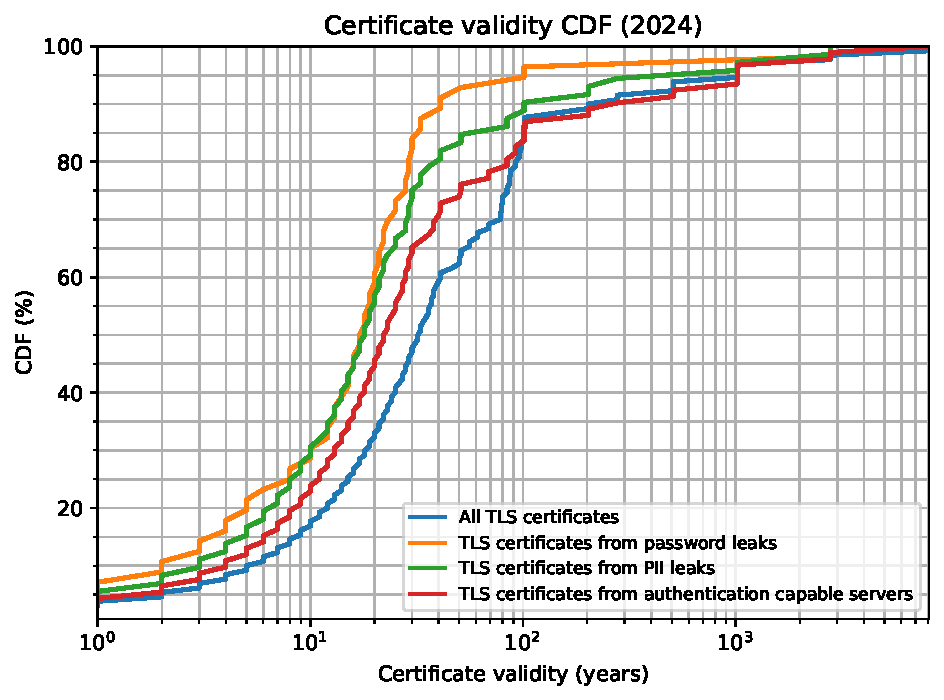
\includegraphics[width=0.45\textwidth]{img/validity_cdf_line.pdf}
    \caption{CDF of TLS certificates validity window}
    \label{fig:certs_validity_window}
\end{figure}
\fi

The use case of \acrshort{LDAP} is often different from that of the Web, which is almost by definition a publicly accessible resource. As data on \acrshort{LDAP} servers may only need to be accessible to very few clients, it is conceivable that an organization operates a custom in-house CA to issue certificates for the \acrshort{LDAP} server and deploys the CA's root certificate only to its clients. Microsoft has tooling for such a purpose, for example. To our analysis, such certificates would appear to have invalid chains as the root CA is not part of any root store. Hence, when we check for valid chains, our numbers are a \textit{lower bound} (and an upper bound for invalid chains).
%We summarize our chain analysis in~\cref{tab:tls_overview}. 
 %The organization's system administrators may want to provide their client's software with a signed and trusted certificate within the organization. We want to highlight that LDAP servers could be accidentally exposed to the Internet, as we discussed in this paper.
Custom CAs can be expected to issue relatively few certificates (as there are few servers per organization).
 
 %by matching the certificate's fingerprints against Mozilla, including \gls{CA}s and intermediary certificates, Common Name, Organisation, and Organisation Unit fields of the X.509 certificate.

 %Although we observed many invalid X.509 chains, we cannot assert that the end-host certificates were signed by its organization \gls{CA} because fields like the common name aren't constrained when issuing an X.509 certificate.
 
 %We investigated the top issuers of globally invalid certificates and found that 21\% were from Let's Encrypt (more precisely, their deprecated R3 instance). We also find ``Philip Newman'' with 9\%, and ``CA'', ``VPN'', ``Certificate Authority'' and Synology accounting with less than 9\% altogether out of 30k invalid chains from our total IPs data set. Besides R3 and Synology, all other issuers are unknown. In summary, we cannot clarify whether such a chain of certificates belongs to a corporation even though this is a valid use case.

\iffalse
\begin{tabular}{lr}
\toprule
Total invalid chains & 39,305 (100\%) \\
\midrule
R3 & 21.19\% \\
Philip Newman & 8.84\% \\
CA & 3.04\% \\
VPN & 2.24\% \\
Certificate Authority & 1.74\% \\
Synology Inc. CA & 1.46\% \\
innovaphone & 1.31\% \\
DOMAIN-VM-OLS-1-CA & 1.25\% \\
Go Daddy Secure Certificate Authority - G2 & 1.03\% \\
www.mail.org & 0.92\% \\
\bottomrule
\label{tab:issuers_invalid_chain}
\caption{End-host X.509 issuers from invalid chains (not only signed by unknown authority) from the view of Total IPs (48,198).}
\end{tabular}
\fi

\paragraph{Common LDAP Clients and Negotiated Cipher Suites.}
To understand what cipher suites common LDAP clients would negotiate, we extracted their list of supported cipher suites from the \textit{Client Hello} messages they send. \cref{tab:ClientHelloCipherSuites} shows the results. This analysis was done several months after our initial scans.


\paragraph{Summarizing View.}

\cref{tab:tls_overview} gives an overview of what we consider \acrshort{TLS} configurations with and without issues, breaking down the reasons into cipher suites (recommended by the RFC vs. others) and certificate chains. We observe that servers that leak credentials or personal data fare worse than the total regarding selected cipher suites and valid X.509 chains.
%Overall, just about a quarter of \acrshort{TLS} connections can be said to have a strong configuration. The number drops substantially in the case of servers that leak credentials (a mere 10\%) or personal data (about 13\%). Servers that leak credentials or store personal data have particularly often poor configurations, both in terms of cipher suites and certificates. 
Furthermore, we verified that cipher suite negotiation that major \gls{LDAP} clients carry out results in very similar results as in our own scans.
The correlation we see between weak cryptography and older \acrshort{TLS} versions on the one hand, and data leakages and vulnerable \acrshort{LDAP} versions on the other hand, would support the hypothesis that the more weakly configured servers have not been updated in several years.

\iffalse
\begin{figure}
    \centering
    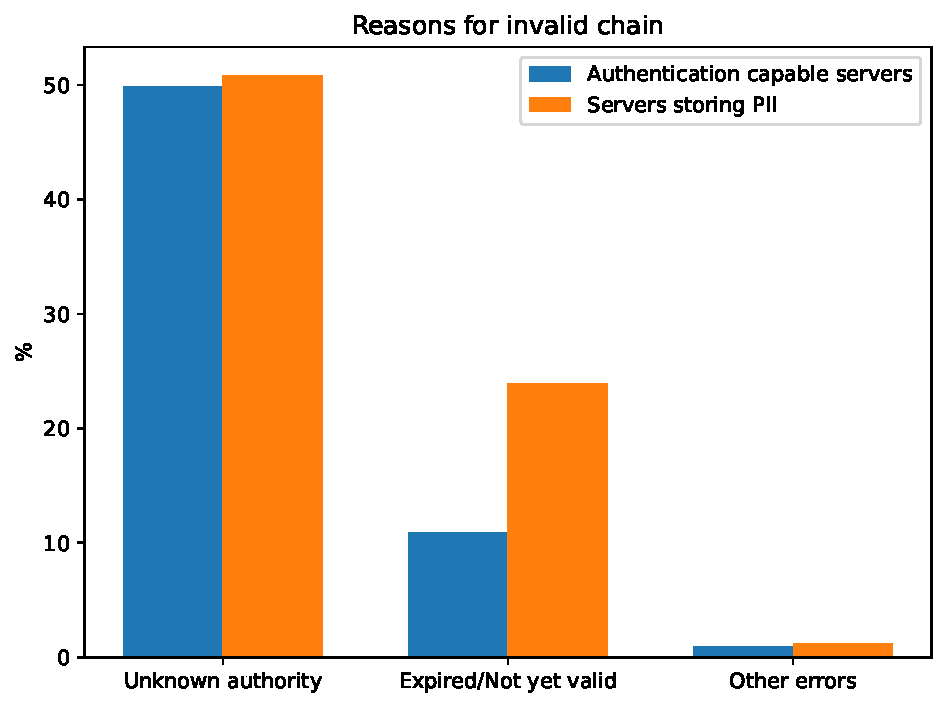
\includegraphics[width=0.45\textwidth]{img/reasons_invalid_chains.pdf}
    \caption{Reasons for invalid X.509 certificate chain.}
    \label{fig:reasons_invalid_chains}
\end{figure}
\fi
